\documentclass{article}
\usepackage{nips12submit_e,bm,amsmath,amsfonts,tikz,amssymb,amsthm,array,todonotes,times}
\usepackage{hyperref}
\usepackage[english]{babel}

\newtheorem{theorem}{Theorem}
\newtheorem{definition}{Definition}

\newcommand{\head}[2]{\multicolumn{1}{>{\centering\arraybackslash}p{#1}}{\textbf{#2}}}
\newcommand{\augx}{\bm \Phi(\bm P(\bm X);k,s)}
\newcommand{\augy}{\bm \Phi(\bm P(\bm Y);k,s)}

\definecolor{MPG}{RGB}{000,125,122}
\newcounter{PHcomment} \newcommand{\PHcomment}[1]{%
  \refstepcounter{PHcomment}%
  { \todo[inline, color={MPG!20},size=\small]{%
      \textbf{Comment [PH \thePHcomment]:}~#1}%
  }}

\title{The Randomized Dependence Coefficient}

\author{
  \textbf{David Lopez-Paz, Philipp Hennig, Bernhard Sch\"olkopf}\\
  Max Planck Institute for Intelligent Systems\\
  Spemannstra{\ss}e 38, T\"ubingen, Germany\\
  \texttt{\{dlopez,phennig,bs\}@tue.mpg.de}
} 

\nipsfinalcopy

\begin{document} 
 
\maketitle 
 
\begin{abstract}
  We introduce the Randomized Dependence Coefficient (RDC), a measure of
  non-linear dependence between random variables of arbitrary dimension based
  on the Hirschfeld-Gebelein-R\'enyi Maximum Correlation Coefficient. RDC is
  defined in terms of correlation of random non-linear copula projections; it
  is invariant with respect to marginal distribution transformations, has low
  computational cost and is easy to implement: just five lines of R code,
  included at the end of the paper.
\end{abstract}

\section{Introduction}\label{sec:intro}
Measuring statistical dependence between random variables is a fundamental
problem in statistics. Commonly used measures of dependence, Pearson's rho,
Spearman's rank or Kendall's tau are computationally efficient and
theoretically well understood, but consider only a limited class of association
patterns, like linear or monotonically increasing functions. The development of
non-linear dependence measures is challenging because of the radically larger
amount of possible association patterns.

Despite these difficulties, many non-linear statistical dependence measures
have been developed recently. Examples include the Alternating Conditional
Expectations or \emph{backfitting algorithm} (ACE) \cite{Breiman85,Hastie86},
Kernel Canonical Correlation Analysis (KCCA) \cite{Bach02}, (Copula)
Hilbert-Schmidt Independence Criterion (CHSIC, HSIC)
\cite{Gretton05,Gretton12,Poczos12}, Distance or Brownian Correlation (dCor)
\cite{Szekely07,Szekely10} and the Maximal Information Coefficient (MIC)
\cite{Reshef11}. However, these methods exhibit high computational demands (at
least quadratic costs in the number of samples for KCCA, HSIC, CHSIC, dCor or
MIC), are limited to measuring dependencies between scalar random variables
(ACE, MIC) or can be difficult to implement (ACE, MIC).

This paper develops the \emph{Randomized Dependence Coefficient} (RDC), an
estimator of the Hirschfeld-Gebelein-R\'enyi Maximum Correlation Coefficient
(HGR) addressing the issues listed above. RDC defines dependence between two
random variables as the largest canonical correlation between random non-linear
projections of their respective empirical copula-transformations. RDC is
invariant to monotonically increasing transformations, operates on random
variables of arbitrary dimension, and has computational cost of $O(n\log n )$
with respect to the sample size.  Moreover, it is easy to implement: just five
lines of R code, included in Appendix \ref{sec:code}.

The following Section reviews the classic work of Alfr\'ed R\'enyi
\cite{Renyi59}, who proposed seven desirable fundamental properties of
dependence measures, proved to be satisfied by the
Hirschfeld-Gebelein-R\'enyi's Maximum Correlation Coefficient (HGR). Section
\ref{sec:rdc} introduces the Randomized Dependence Coefficient as an estimator
designed in the spirit of HGR, since HGR itself is computationally intractable.
Properties of RDC and its relationship to other non-linear dependence measures
are analysed in Section \ref{sec:rdc_prop}. Section \ref{sec:exps} validates
the empirical performance of RDC on a series of numerical experiments on both
synthetic and real-world data.

\section{Hirschfeld-Gebelein-R\'enyi's Maximum Correlation
Coefficient}\label{sec:renyi}
In 1959 \cite{Renyi59}, Alfr\'ed R\'enyi argued that a measure of dependence
$\rho^* : \mathcal{X} \times \mathcal{Y} \rightarrow [0,1]$ between random
variables $X\in\mathcal{X}$ and $Y\in\mathcal{Y}$ should satisfy seven
fundamental properties:
\begin{enumerate}
  \item $\rho^*(X,Y)$ is defined for any pair of non-constant random variables
  $X$ and $Y$.
  \item $\rho^*(X,Y) = \rho^*(Y,X)$
  \item $0 \leq \rho^*(X,Y) \leq 1$
  \item $\rho^*(X,Y) = 0$ iff $X$ and $Y$ are statistically independent.
  \item For bijective  Borel-measurable functions $f,g : \mathbb{R}
  \rightarrow \mathbb{R}$, $\rho^*(X,Y) = \rho^*(f(X),g(Y))$.
  \item $\rho^*(X,Y) = 1$ if for Borel-measurable functions $f$ or $g$, $Y =
  f(X)$ or $X = g(Y)$.
  \item If $(X,Y) \sim \mathcal{N}(\bm \mu, \bm \Sigma)$, then $\rho^*(X,Y) =
  |\rho(X,Y)|$, where $\rho$ is the correlation coefficient.
\end{enumerate}
R\'enyi also showed the \emph{Hirschfeld-Gebelein-R\'enyi Maximum
  Correlation Coefficient} (HGR) \cite{Gebelein41,Renyi59} to satisfy
all these properties. HGR was defined by Gebelein in 1941
\cite{Gebelein41} as the supremum of Pearson's correlation coefficient
$\rho$ over all Borel-measurable functions $f,g$ of finite variance:
\begin{equation}\label{eq:hgr}
  \text{hgr}(X,Y) = \sup_{f,g} \rho(f(X),g(Y)),
\end{equation}
Since the supremum in \eqref{eq:hgr} is over an infinite-dimensional
space, HGR is not computable. It is an abstract concept, not a
practical dependence measure. In the following we propose a scalable
estimator with the same structure as HGR: the Randomized Dependence
Coefficient.

\section{Randomized Dependence Coefficient} \label{sec:rdc} 
The \emph{Randomized Dependence Coefficient} (RDC) measures the dependence
between random samples $\bm X \in \mathbb{R}^{p\times n}$ and $\bm Y \in
\mathbb{R}^{q\times n}$ as the largest canonical correlation between $k$
randomly chosen non-linear projections of their copula transformations. Before
Section~\ref{sec:formal-definition-or} defines this concept formally, we
describe the three necessary steps to construct the RDC statistic:
copula-transformation of each of the two random samples
(Section~\ref{sec:estim-copula-transf}), projection of the copulas through $k$
randomly chosen non-linear maps (Section~\ref{sec:gener-rand-non}) and
computation of the largest canonical correlation between the two sets of
non-linear random projections (Section~\ref{sec:comp-canon-corr}). Figure
\ref{fig:rdcsteps} offers a sketch of this process.
\begin{figure}[h!]
  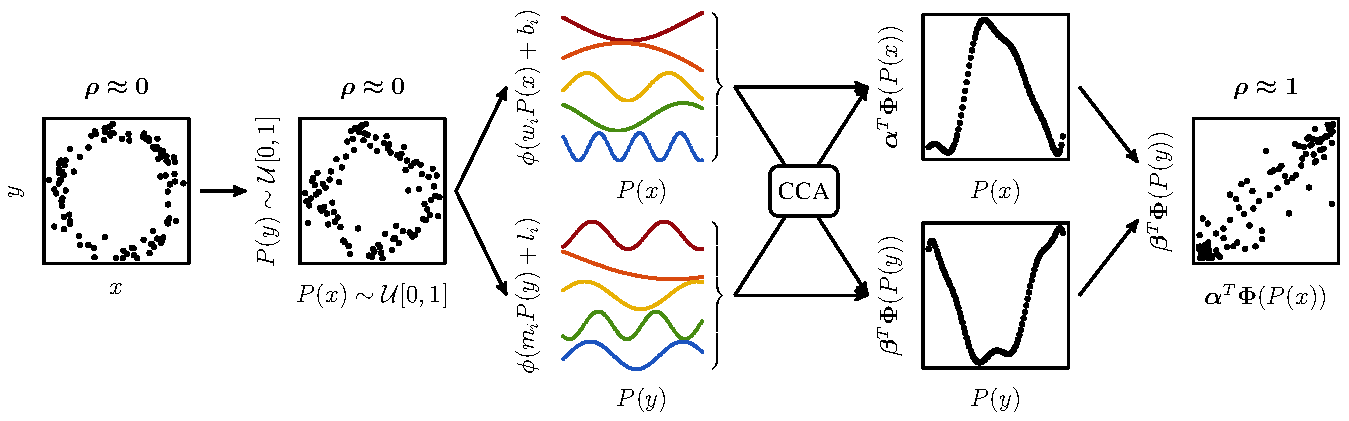
\includegraphics[width=\textwidth]{figures/pipeline.pdf}
  \caption{RDC computation for a simple set of samples
  $\{(x_i,y_i)\}_{i=1}^{100}$ drawn from a noisy circular pattern: The samples
  are used to estimate the copula, then mapped with randomly drawn non-linear
  functions. The RDC is the largest canonical correlation between these
  non-linear projections.}
  \label{fig:rdcsteps}
\end{figure}

\subsection{Estimation of Copula-Transformations}
\label{sec:estim-copula-transf}
To achieve invariance with respect to transformations on marginal distributions
(such as shifts or rescalings), we operate on the \emph{empirical copula
transformation} of the data \cite{Nelsen06,Poczos12}. Consider a random vector
$\bm X = (X_1, \ldots, X_d)$ with continuous marginal cumulative distribution
functions (cdfs) $P_i$, $1 \leq i \leq d$. Then the vector $\bm U =
(U_1,\ldots,U_d) := \bm P(\bm X) = (P_1(X_1),\ldots,P_d(X_d))$, known as the
\emph{copula transformation}, has uniform marginals:
\begin{theorem}
  (Probability Integral Transform \cite{Nelsen06}) For a random variable $X$
  with cdf $P$, the random variable $U := P(X)$ is uniformly distributed on
  $[0,1]$.
\end{theorem}
The random variables $U_1, \ldots, U_d$ are known as the observation ranks of
$X_1, \ldots, X_d$. Crucially, $\bm U$ preserves the dependence structure of
the original random vector $\bm X$, but ignores each of its $d$ marginal forms
\cite{Nelsen06}.  The joint distribution of $\bm U$ is known as the copula of
$\bm X$:
\begin{theorem}
  (Sklar \cite{Sklar59}) Let the random vector $\bm X = (X_1, \ldots, X_d)$
  have continuous marginal cdfs $P_i$, $1 \leq i \leq d$. Then, the joint
  cumulative distribution of $\bm X$ is uniquely expressed as:
\begin{equation}
  P(X_1, \ldots, X_d) = C(P_1(X_1), \ldots, P_d(X_d)),
\end{equation}
where the distribution $C$ is known as the copula of $\bm X$.
\end{theorem}
A practical estimator of the univariate cdfs $P_1, \ldots, P_d$ is the
\emph{empirical cdf}:
\begin{equation}
  P_n(x) := \frac{1}{n} \sum_{i=1}^n \mathbb{I}(X_i \leq x),
\end{equation}
which gives rise to the \emph{empirical copula transformations} of a
multivariate sample:
\begin{equation}
\bm P_n(\bm x) = [{P}_{n,1}(x_1), \ldots, {P}_{n,d}(x_d)].
\end{equation}
The Massart-Dvoretzky-Kiefer-Wolfowitz inequality \cite{Massart90} can be used
to show that empirical copula transformations converge fast to the true
transformation as the sample size increases:
\begin{theorem}
  (Convergence of the empirical copula, \cite[Lemma 7]{Poczos12}) Let $\bm X_1,
  \ldots, \bm X_n$ be an i.i.d. sample from a probability distribution over
  $\mathbb{R}^d$ with marginal cdf's $P_1, \ldots, P_d$. Let $\bm P(\bm X)$ be
  the copula transformation and $\bm P_n(\bm X)$ the empirical copula
  transformation. Then, for any $\epsilon > 0$:
    \begin{equation}
      \Pr \left[ \sup_{\bm x \in \mathbb{R}^d} \| \bm P(\bm x) - \bm P_n(\bm x)
      \|_2 > \epsilon \right] \leq 2 d \exp \left( -\frac{2 n
      \epsilon^2}{d}\right).
    \end{equation}
\end{theorem}
Computing $\bm P_n(\bm X)$ involves sorting the marginals of $\bm X \in
\mathbb{R}^{d\times n}$, thus $O(d n \log (n))$ operations.

\subsection{Generation of Random Non-Linear Projections}
\label{sec:gener-rand-non}
The second step of the RDC computation is to augment the empirical copula
transformations with non-linear projections, so that linear methods can
subsequently be used to capture non-linear dependencies on the original data.
This is a classic idea also used in other areas, particularly in regression. In
an elegant result, Rahimi and Recht \cite{Rahimi08} proved that linear
regression on random, non-linear projections of the original feature space can
generate high-performance regressors:
\begin{theorem}\label{thm:rahimi}
(Rahimi-Recht) 
Let $p$ be a distribution on $\Omega$ and $|\phi(\bm x; \bm w)| \leq 1$.
%
Let $\mathcal{F} = \left\lbrace \left. f(\bm x) = \int_\Omega
    \alpha(\bm w) \phi(\bm x; \bm w) \mathrm{d}\bm w \right|
  |\alpha(\bm w)| \leq C p(\bm w)\right\rbrace$.
%
Draw $\bm w_1, \ldots, \bm w_k$ iid from $p$.
%
Further let $\delta > 0$, and $c$ be some $L$-Lipschitz loss function,
and consider data $\{\bm x_i, y_i\}_{i=1}^n$ drawn iid from some
arbitrary $P(\bm X,Y)$. The $\alpha_1, \ldots, \alpha_k$ for which
${f}_k(\bm x) = \sum_{i=1}^k \alpha_i \phi(\bm x; \bm w_i)$ minimizes
the empirical risk $c(f_k(\bm x),y)$ has a distance from the $c$-optimal
estimator in $\mathcal{F}$ bounded by
\begin{equation}
 \mathbb{E}_P[c({f}_k(\bm x),y)] - \min_{f\in \mathcal{F}}
 \mathbb{E}_P[c(f(\bm x),y)] \leq O\left(\left( \frac{1}{\sqrt{n}} +
 \frac{1}{\sqrt{k}} \right) LC\sqrt{\log \frac{1}{\delta}}\right)
\end{equation}
with probability at least $1-2\delta$.
\end{theorem}
Intuitively, Theorem \ref{thm:rahimi} states that randomly selecting $\bm w_i$
in $\sum_{i=1}^k \alpha_i \phi(\bm x; \bm w_i)$ instead of optimising them
causes only bounded error.

The choice of the non-linearities $\phi : \mathbb{R} \rightarrow \mathbb{R}$ is
the main and unavoidable assumption in RDC. This choice is a
well-known problem common to all non-linear regression methods and has been
studied extensively in the theory of regression as the selection of reproducing
kernel Hilbert space \cite[\textsection3.13]{learningwithkernels}.  The only
way to favour one such family and distribution over another is to use prior
assumptions about which kind of distributions the method will typically have to
analyse. 

We use random features instead of the Nystr\"om method because of their smaller
memory and computation requirements \cite{Le13}.  In our experiments, we will
use sinusoidal projections, $\phi(\bm w^T \bm x +b) := \sin(\bm w^T \bm x +
b)$.  Arguments favouring this choice are that shift-invariant kernels are
approximated with these features when using the appropriate random parameter
sampling distribution \cite{Rahimi08},
\cite[p.~208]{gihman4s:_theor_stoch_proces}
\cite[p.~24]{stein99:_inter_spatial_data}, and that functions with absolutely
integrable Fourier transforms are approximated with $L_2$ error below
$O(1/\sqrt{k})$ by $k$ of these features \cite{Jones92}.

Let the random parameters $\bm w_i \sim \mathcal{N}(\bm 0, s\bm I)$, $b_i \sim
\mathcal{N}(0, s)$. Choosing $\bm w_i$ to be Normal is analogous to the use of
the Gaussian kernel for HSIC, CHSIC or KCCA \cite{Rahimi08}.  Tuning $s$ is
analogous to selecting the kernel width, that is, to regularize the
non-linearity of the random projections.

Given a data collection $\bm X = (\bm x_1, \ldots, \bm x_n)$, we will denote by
\begin{equation}
  \bm \Phi(\bm X; k,s) := 
  \left(
  \begin{array}{ccc}
  \phi(\bm w_1^T \bm x_1+b_1) & \cdots & \phi(\bm w_k^T \bm x_1+b_k)\\
  \vdots & \vdots & \vdots \\
  \phi(\bm w_1^T \bm x_n+b_1) & \cdots & \phi(\bm w_k^T \bm x_n +b_k)
  \end{array}
  \right)^T
\end{equation}
the $k-$th order random non-linear projection from $\bm X \in \mathbb{R}^{d
\times n}$ to $\bm \Phi(\bm X; k, s) \in
\mathbb{R}^{k \times n}$. The computational complexity of computing $\bm
\Phi(\bm X; k, s)$ with naive matrix multiplications is $O(kdn)$. However,
recent techniques using fast Walsh-Hadamard transforms \cite{Le13} allow
computing these feature expansions within a computational cost of
$O(k\log(d)n)$ and $O(k)$ storage.

\subsection{Computation of Canonical Correlations} \label{sec:comp-canon-corr}
The final step of RDC is to compute the linear combinations of the augmented
empirical copula transformations that have maximal correlation. Canonical
Correlation Analysis (CCA, \cite{Haerdle07}) is the calculation of pairs of
basis vectors $(\bm \alpha, \bm \beta)$ such that the projections $\bm \alpha^T
\bm X$ and $\bm \beta^T \bm Y$ of two random samples $\bm X \in
\mathbb{R}^{p\times n}$ and $\bm Y \in \mathbb{R}^{q\times n}$ are maximally
correlated. The correlations between the projected (or canonical) random
samples are referred to as canonical correlations. There exist up to
$\max(\text{rank}(\bm X), \text{rank}(\bm Y))$ of them. Canonical correlations
$\rho^2$ are the solutions to the eigenproblem:
\begin{align}
  \left(
    \begin{array}{cc}
    \bm 0 & \bm C_{xx}^{-1}\bm C_{xy}\\
    \bm C_{yy}^{-1}\bm C_{yx} & \bm 0
    \end{array}
  \right)
  \left(
    \begin{array}{c}
    \bm \alpha\\
    \bm \beta 
    \end{array}
  \right)
  =
  \rho^2
  \left(
    \begin{array}{c}
    \bm \alpha\\
    \bm \beta 
    \end{array}
  \right)
  ,\label{eq:eigenset}
\end{align}
where $\bm C_{xy} = \text{cov}(\bm X, \bm Y)$ and the matrices $\bm C_{xx}$ and
$\bm C_{yy}$ are assumed to be invertible. Therefore, the largest canonical
correlation $\rho_1$ between $\bm X$ and $\bm Y$ is the supremum of the
correlation coefficients over their linear projections, that is:
$  \rho_1(\bm X, \bm Y) = \sup_{\bm \alpha, \bm \beta} \rho(\bm \alpha^T \bm X,
  \bm \beta^T \bm Y).
$

When $p,q \ll n$, the cost of CCA is dominated by the estimation of the matrices $\bm
C_{xx}$, $\bm C_{yy}$ and $\bm C_{xy}$, hence being $O((p+q)^2n)$ for two
random variables of dimensions $p$ and $q$, respectively.

\subsection{Formal Definition or RDC}
\label{sec:formal-definition-or}
Given the random samples $\bm X \in \mathbb{R}^{p\times n}$ and $\bm Y \in
\mathbb{R}^{q\times n}$ and the parameters $k \in \mathbb{N}_+$ and $s \in
\mathbb{R}_+$, the Randomized Dependence Coefficient between $\bm X$ and $\bm
Y$ is defined as:
\begin{equation}\label{eq:rdc}
  \text{rdc}(\bm X, \bm Y; k,s) :=
  \sup_{\bm \alpha, \bm \beta}\rho\left(
  \bm \alpha^T \bm \Phi(\bm P(\bm X); k, s),
  \bm \beta^T \bm \Phi(\bm P(\bm Y); k, s)\right).
\end{equation}

\section{Properties of RDC}\label{sec:rdc_prop}
\paragraph{Computational complexity:} In the typical setup (very large $n$,
large $p$ and $q$, small $k$) the computational complexity of RDC is dominated
by the calculation of the copula-transformations. Hence, we achieve a cost in
terms of the sample size of $O((p+q) n \log n + kn\log(pq) + k^2n) \approx O(n
\log n)$. 

\paragraph{Ease of implementation:} An implementation of RDC in R is included
in the Appendix \ref{sec:code}.

\paragraph{Relationship to the HGR coefficient:} \label{sec:relat-hgr}
It is tempting to wonder whether RDC is a consistent, or even an efficient
estimator of the HGR coefficient. However, a simple experiment shows
that it is not desirable to approximate HGR exactly on finite datasets:
Consider $p(X,Y)=\mathcal{N}(x;0,1)\mathcal{N}(y;0,1)$ which is independent,
thus, by both R\'enyi's 4th and 7th properties, has $\mathrm{hgr}(X,Y)=0$.
However, for finitely many $N$ samples from $p(X,Y)$, almost surely, values in
both $X$ and $Y$ are pairwise different and separated by a finite difference.
So there exist continuous (thus Borel measurable) functions $f(X)$ and $g(Y)$
mapping both $X$ and $Y$ to the sorting ranks of $Y$, i.e.
$f(x_i)=g(y_i)\;\forall (x_i,y_i)\in(\bm X,\bm Y)$. Therefore, the
finite-sample version of Equation \eqref{eq:hgr} is constant and equal to ``1'' 
for continuous random variables. Meaningful measures of dependence from finite
  samples thus must rely on some form of regularization. RDC achieves this by
  approximating the space of Borel measurable functions with the restricted
  function class $\mathcal{F}$ from Theorem \ref{thm:rahimi}:

Assume the optimal transformations $f$ and $g$ (Equation 1) to belong to the
Reproducing Kernel Hilbert Space $\mathcal{F}$ (Theorem 4), with associated
shift-invariant, positive semi-definite kernel function $k(\bm x, \bm x') =
\langle \bm \phi(\bm x), \bm \phi(\bm x')\rangle_\mathcal{F} \leq 1$. Then, with
probability greater than $1-2\delta$:
\begin{equation}
\label{eq:err_total}
\mathrm{hgr}(\bm X, \bm Y; \mathcal{F}) - 
\mathrm{rdc}(\bm X, \bm Y; k) 
= O\left(\left(\frac{\|\bm
m\|_F}{\sqrt{n}}+\frac{LC}{\sqrt{k}}\right)
 \sqrt{\log\frac{1}{\delta}}\right),\end{equation}
where $\bm m := \bm \alpha \bm \alpha^T +\bm \beta \bm \beta^T$ and $n$, $k$
denote the sample size and number of random features. The bound
(\ref{eq:err_total}) is the sum of two errors. The error $O(1/\sqrt{n})$ is due
to the convergence of CCA's largest eigenvalue in the finite sample size
regime.  This result \cite[Theorem 6]{Hardoon09} is originally obtained by
posing CCA as a least squares regression on the product space induced by the
feature map $\bm \psi(\bm x, \bm y) = [\bm \phi(\bm x)\bm \phi(\bm x)^T, \bm
\phi(\bm y) \phi(\bm y)^T, \sqrt{2}\bm \phi(\bm x) \phi(\bm y)^T]^T$.  Because of
approximating $\bm \psi$ with $k$ random features, an additional error 
$O(1/\sqrt{k})$ is introduced in the least squares regression \cite[Lemma
3]{Rahimi08}. Therefore, an equivalence between RDC and KCCA is established if
RDC uses an infinite number of sinusoidal features, the random sampling distribution is
set to the inverse Fourier transform of the shift-invariant kernel used by KCCA and
the copula-transformations are discarded.
However, when $k \geq n$ regularization
is needed to avoid spurious perfect correlations, as discussed above.

\paragraph{Relationship to other estimators:}\label{sec:comparison} Table
\ref{table:comparison} summarizes several state-of-the-art dependence measures
showing, for each measure, whether it allows for general non-linear dependence
estimation, handles multidimensional random variables, is invariant with
respect to changes in marginal distributions, returns a statistic in $[0,1]$,
satisfy R\'enyi's properties (Section \ref{sec:renyi}), and how many parameters
it requires. As parameters, we here count the kernel function for kernel
methods, the basis function and number of random features for RDC, the stopping
tolerance for ACE and the search-grid size for MIC, respectively. Finally, the
table lists computational complexities with respect to sample size.

When using random features $\phi$ linear for some neighbourhood around zero
(like sinusoids or sigmoids), RDC converges to Spearman's rank correlation
coefficient as $s \rightarrow 0$, for any $k$.

\begin{table}[h!]
  \caption{Comparison between non-linear dependence measures.}
  \vskip 0.3 cm
\resizebox{\textwidth}{!}
{
  \begin{tabular}{lccccccl}
  \hline
  \head{1.5cm}{\textbf{Name of Coeff.}}     &
  \head{ .9cm}{\textbf{Non-Linear}}         &
  \head{1.2cm}{\textbf{Vector Inputs}}      &
  \head{1.6cm}{\textbf{Marginal Invariant}} & 
  \head{1.9cm}{\textbf{Renyi's Properties}} &
  \head{1.1cm}{Coeff. \textbf{$\in [0,1]$}} &
  \head{1cm}{\# \textbf{Par.}}         &
  \head{1cm}{\textbf{Comp. Cost}}\\\hline\hline
  Pearson's $\rho$      & $\times$     & $\times$     & $\times$     & $\times$     & $\checkmark$ & 0 & $n$        \\ \hline
  Spearman's $\rho$     & $\times$     & $\times$     & $\checkmark$ & $\times$     & $\checkmark$ & 0 & $n \log n$ \\ \hline
  Kendall's $\tau$      & $\times$     & $\times$     & $\checkmark$ & $\times$     & $\checkmark$ & 0 & $n \log n$ \\ \hline
  CCA                   & $\times$     & $\checkmark$ & $\times$     & $\times$     & $\checkmark$ & 0 & $n$     \\ \hline
  KCCA \cite{Bach02}    & $\checkmark$ & $\checkmark$ & $\times$     & $\times$     & $\checkmark$ & 1 & $n^3$      \\ \hline
  ACE  \cite{Breiman85} & $\checkmark$ & $\times$     & $\times$     & $\checkmark$ & $\checkmark$ & 1 & $n$   \\ \hline
  MIC  \cite{Reshef11}  & $\checkmark$ & $\times$     & $\times$     & $\times$     & $\checkmark$ & 1 & $n^{1.2}$      \\ \hline
  dCor \cite{Szekely07} & $\checkmark$ & $\checkmark$ & $\times$     & $\times$     & $\checkmark$ & 1 & $n^2$      \\ \hline
  HSIC \cite{Gretton12}  & $\checkmark$ & $\checkmark$ & $\times$     & $\times$     & $\times$     & 1 & $n^2$      \\ \hline
  CHSIC \cite{Poczos12}  & $\checkmark$ & $\checkmark$ & $\checkmark$ & $\times$     & $\times$     & 1 & $n^2$      \\ \hline
  \textbf{RDC}          & $\checkmark$ & $\checkmark$ & $\checkmark$ & $\checkmark$ & $\checkmark$ & 2 & $n \log n$ \\ \hline\hline
  \end{tabular}
}
\label{table:comparison}
\end{table}

\paragraph{Testing for independence with RDC:} Consider the hypothesis ``the
two sets of non-linear projections are mutually uncorrelated''.  Under
normality assumptions (or large sample sizes), Bartlett's approximation
\cite{Mardia79} can be used to show
$
  \left(\frac{2k+3}{2}-n\right) \log \prod_{i=1}^k (1-\rho_i^2) \sim
  \chi^2_{k^2}
$,
where $\rho_1, \ldots, \rho_k$ are the canonical correlations between  $\augx$
and $\augy$. Alternatively, non-parametric asymptotic distributions can be
obtained from the spectrum of the inner products of the non-linear random
projection matrices \cite[Theorem 3]{Zhang12}.

\section{Experimental Results}\label{sec:exps}
We performed experiments on both synthetic and real-world data to validate the
empirical performance of RDC versus the non-linear dependence measures listed
in Table \ref{table:comparison}. In some experiments we do not compare against
to KCCA because we were unable to find a good set of hyperparameters.

\paragraph{Parameter selection:} For RDC, the number of random features is set
to $k=20$ for both random samples, since no significant improvements were
observed for larger values.  The random feature sampling parameter $s$ is more
crucial, and set as follows: when the marginals of $\bm u$ are standard
uniforms, $\bm w \sim \mathcal{N}(\bm 0, s \bm I)$ and $b \sim
\mathcal{N}(0,s)$, then $\mathbb{V}[\bm w^T \bm u + b] = s\left(1+\frac{d}{3}
\right)$; therefore, we opt to set $s$ to a linear scaling of the input
variable dimensionality.  In all our experiments $s = \frac{1}{6d}$ worked
well. The development of better methods to set the parameters of RDC is left as
future work.

HSIC and CHSIC use Gaussian kernels $k(\bm z, \bm z') = exp(-\gamma\| \bm z-
\bm z'\|_2^2)$ with $\gamma^{-1}$ set to the euclidean distance median of each
sample \cite{Gretton12}. MIC's search-grid size is set to $B(n) = n^{0.6}$ as
recommended by the authors \cite{Reshef11}, although speed improvements are
achieved when using lower values. ACE's tolerance is set to $\epsilon = 0.01$,
default value in the R package \texttt{acepack}.
\subsection{Synthetic Data}

\paragraph{Resistance to additive noise:}
We define the \emph{power} of a dependence measure as its ability to discern
between dependent and independent samples that share equal marginal forms. In
the spirit of Simon and
Tibshirani\footnote{\url{http://www-stat.stanford.edu/~tibs/reshef/comment.pdf}},
we conducted experiments to estimate the power of RDC as a measure of
non-linear dependence.  We chose 8 bivariate association patterns, depicted
inside little boxes in Figure \ref{fig:power}. For each of the 8 association
patterns, 500 repetitions of 500 samples were generated, in which the input
sample was uniformly distributed on the unit interval. Next, we regenerated
the input sample randomly, to generate independent versions of each sample
with equal marginals. Figure \ref{fig:power} shows the power for the discussed
non-linear dependence measures as the variance of some zero-mean Gaussian
additive noise increases from $1/30$ to $3$.  RDC shows worse performance in
the linear association pattern due to overfitting and in the
step-function due to the smoothness prior induced by the sinusoidal
features, but has good performance in non-functional association
patterns.

\paragraph{Running times:}
Table \ref{fig:times} shows running times for the considered non-linear
dependence measures on scalar, uniformly distributed, independent samples of
sizes $\{10^3, \ldots, 10^6\}$ when averaging over 100 runs. Single runs above
ten minutes were cancelled. Pearson's $\rho$, ACE, dCor, KCCA and MIC are
implemented in C, while RDC, HSIC and CHSIC are implemented as interpreted R
code. KCCA is approximated using incomplete Cholesky decompositions as described
in \cite{Bach02}.

\begin{table}[h!]
  \caption{Average running times (in seconds) for dependence measures on
  versus sample sizes.}
  \vskip 0.3 cm
    \resizebox{\textwidth}{!}{
    \begin{tabular}{l|cccccccc}
    \hline
   \bf sample size& \bf Pearson's $\rho$ & \bf RDC       & \bf ACE       & \bf KCCA & \bf  dCor     & \bf HSIC     & \bf CHSIC    & \bf MIC      \\\hline\hline
    1,000     & 0.0001  & 0.0047   &  0.0080   &  0.402  &  0.3417  & 0.3103  &  0.3501 & 1.0983 \\\hline
    10,000    & 0.0002  & 0.0557   &  0.0782   &  3.247  &  59.587  & 27.630  &  29.522 &  ---   \\\hline
    100,000   & 0.0071  & 0.3991   &  0.5101   &  43.801 &  ---     &  ---    &  ---    &  ---   \\\hline
    1,000,000 & 0.0914  & 4.6253   &  5.3830   &  ---    &  ---     &  ---    &  ---    &  ---    \\\hline
    \hline
    \end{tabular}
  }
\label{fig:times}
\end{table}

\paragraph{Value of statistic in $[0,1]$:} Figure \ref{fig:pairs} shows RDC,
ACE, dCor, MIC, Pearson's $\rho$, Spearman's rank and Kendall's $\tau$
dependence estimates for 14 different associations of two scalar random
samples.  RDC scores values close to one on all the proposed dependent
associations, whilst scoring values close to zero for the independent
association, depicted last.  When the associations are Gaussian (first row),
RDC scores values close to the Pearson's correlation coefficient
%, as suggested in the seventh property of R\'enyi
(Section \ref{sec:renyi}, 7th property).

\subsection{Feature Selection in Real-World Data} We performed greedy feature
selection via dependence maximization \cite{Song12} on eight real-world
datasets. More specifically, we attempted to construct the subset of features
$\mathcal{G} \subset \mathcal{X}$ that minimizes the normalized mean squared
regression error (NMSE) of a Gaussian process regressor. We do so by selecting
the feature $x^{(i)}$ maximizing dependence between the feature set
$\mathcal{G}_{i} = \{\mathcal{G}_{i-1} , x^{(i)}\}$ and the target variable $y$
at each iteration $i \in \{1, \ldots 10\}$, such that $\mathcal{G}_0 = \{
  \emptyset \}$ and $x^{(i)} \notin \mathcal{G}_{i-1}$.

We considered 12 heterogeneous datasets, obtained from the UCI dataset
repository\footnote{\url{http://www.ics.uci.edu/~mlearn}}, the Gaussian process
web site Data\footnote{\url{http://www.gaussianprocess.org/gpml/data/}} and the
Machine Learning data set repository\footnote{\url{http://www.mldata.org}}.
Random training/test partitions are computed to be disjoint and equal sized.

Since $\mathcal{G}$ can be multi-dimensional, we compare RDC to the non-linear
methods dCor, HSIC and CHSIC. Given their quadratic computational demands, dCor,
HSIC and CHSIC use up to $1,000$ points when measuring dependence; this
constraint only applied on the \texttt{sarcos} and \texttt{abalone} datasets.
Results are averages of $20$ random training/test partitions.

\begin{figure}[h!]
  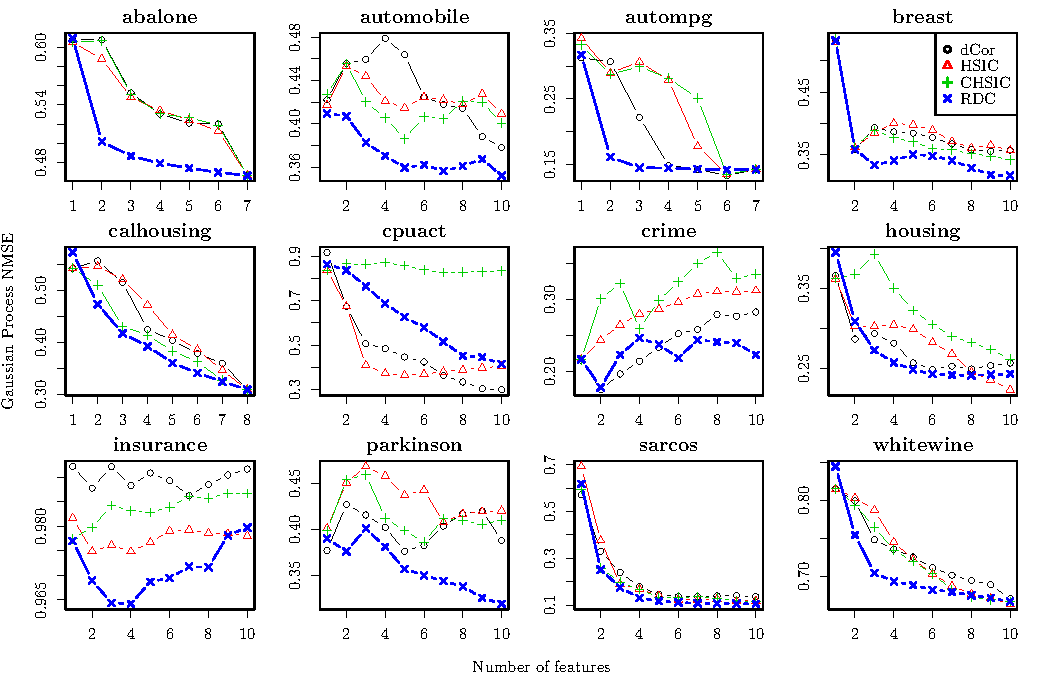
\includegraphics[width=\textwidth]{figures/real_sin.pdf}
  \caption{Feature selection experiments on real-world datasets.}
  \label{fig:featsel}
\end{figure}

Figure \ref{fig:featsel} summarizes the results for all datasets and algorithms
as the number of selected features increases. RDC performs best in most
datasets, with much lower running time than its
contenders.

\section{Conclusion}
\label{sec:conclusion}

We have presented the randomized dependence coefficient, a lightweight
non-linear measure of dependence between multivariate random samples.
Constructed as a finite-dimensional estimator in the spirit of the
Hirschfeld-Gebelein-R\'enyi maximum correlation coefficient, RDC performs well
empirically, is scalable to very large datasets, and is easy to adapt to concrete
problems. 

We thank fruitful discussions with Alberto
Su\'arez, Theofanis Karaletsos and David Reshef.

\newpage
\clearpage
\begin{figure}[t!]
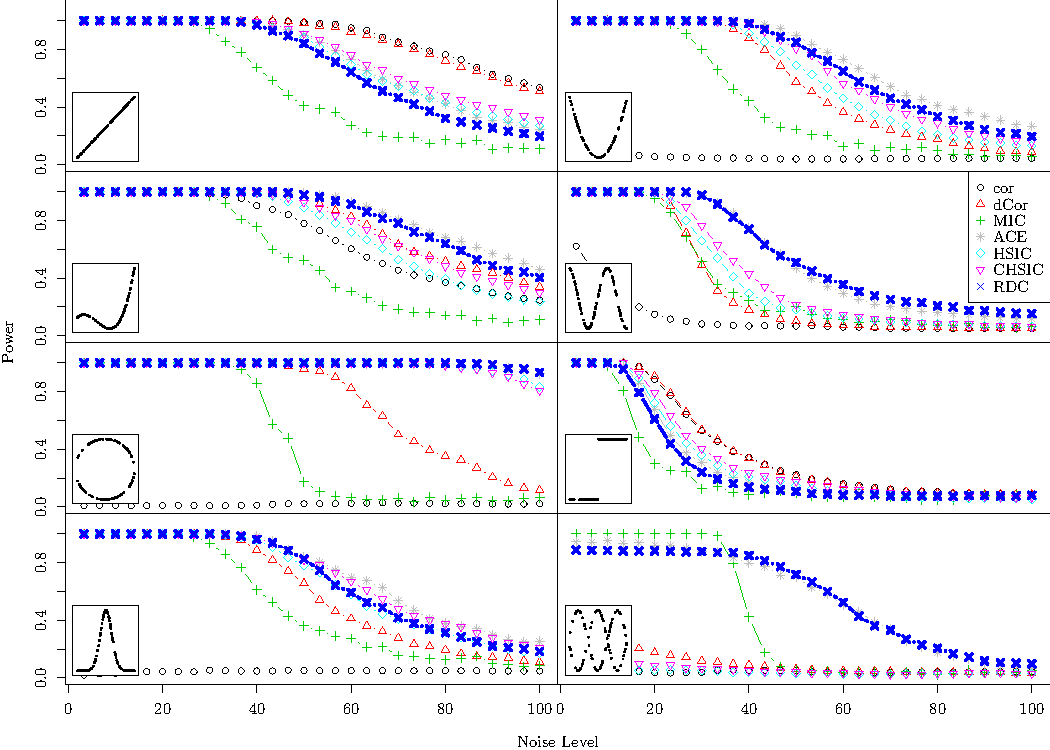
\includegraphics[width=\textwidth]{figures/power_sin.pdf}
\caption{Power of discussed measures on several bivariate association patterns
as noise increases. Insets show the noise-free form of each association
pattern.}
\label{fig:power}
\end{figure}

\begin{figure}[h!]
\centering
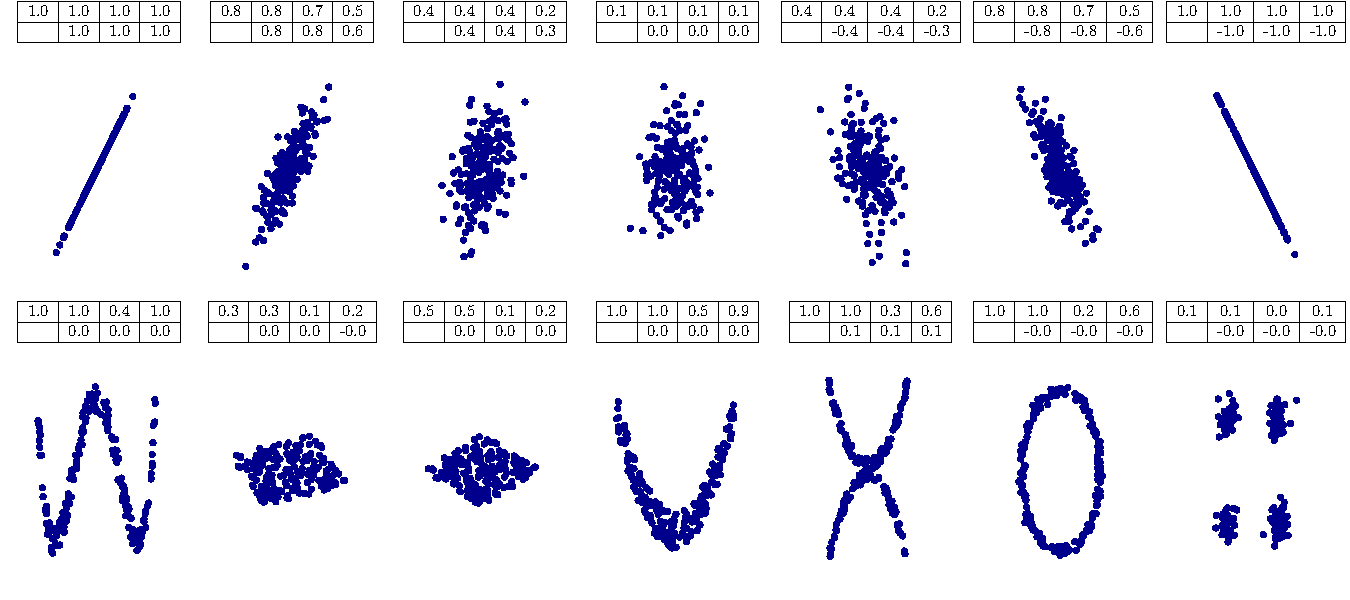
\includegraphics[width=\textwidth]{figures/pairs.pdf}
\vskip -.5 cm
\caption{RDC, ACE, dCor, MIC, Pearson's $\rho$, Spearman's rank and Kendall's
$\tau$ estimates (numbers in tables above plots, in that order) for several
bivariate association patterns.}
\label{fig:pairs}
\end{figure}


\appendix
\section{R Source Code}\label{sec:code}
\begin{small}
\begin{verbatim}rdc <- function(x,y,k=20,s=1/6,f=sin) {
  x <- cbind(apply(as.matrix(x),2,function(u)rank(u)/length(u)),1)
  y <- cbind(apply(as.matrix(y),2,function(u)rank(u)/length(u)),1)
  x <- s/ncol(x)*x%*%matrix(rnorm(ncol(x)*k),ncol(x))
  y <- s/ncol(y)*y%*%matrix(rnorm(ncol(y)*k),ncol(y))
  cancor(cbind(f(x),1),cbind(f(y),1))$cor[1]
}
\end{verbatim}
\end{small}

\newpage
\clearpage
\bibliography{nips2013_rdc}
\bibliographystyle{plain}
\end{document}
